%% main_report47.tex
%% SAMBP TR-47/2026: Feature Engineering and Physics Constraints for ML Protection
%%
%% pdflatex main_report47.tex

\documentclass[11pt,a4paper]{article}

\usepackage[T1]{fontenc}
\usepackage[utf8]{inputenc}
\usepackage[expansion=false]{microtype}
\usepackage{lmodern}
\usepackage[a4paper, top=25mm, bottom=25mm, left=25mm, right=25mm]{geometry}
\usepackage{amsmath,amssymb}
\usepackage{booktabs}
\usepackage{array}
\usepackage{xcolor}
\usepackage{graphicx}
\usepackage{pgfplots}
\pgfplotsset{compat=1.18}
\usepackage{tikz}
\usetikzlibrary{arrows.meta,shapes.geometric,positioning,fit,calc,decorations.pathreplacing}
\usepackage{hyperref}
\usepackage[numbers,sort&compress]{natbib}

\definecolor{sambpblue}{RGB}{0,70,140}

\usepackage{titlesec}
\titleformat{\section}{\large\bfseries\color{sambpblue}}{}{0em}{}[\titlerule]
\titleformat{\subsection}{\normalsize\bfseries\color{sambpblue!80}}{}{0em}{}

\usepackage{fancyhdr}
\pagestyle{fancy}
\fancyhf{}
\rhead{\small\color{gray} SAMBP TR-47/2026}
\lhead{\small\color{gray} Feature Engineering for ML Protection}
\cfoot{\small\thepage}

\begin{document}

\begin{center}
  {\LARGE\bfseries\color{sambpblue} SAMBP Technical Report TR-47/2026}\\[6pt]
  {\large Feature Engineering and Physics Constraints\\
    for ML Protection}\\[10pt]
  {\normalsize PhD Thesis Supporting Report \quad|\quad 2026}
\end{center}

\vspace{2pt}\hrule\vspace{8pt}

\begin{abstract}
\noindent
This report performs a systematic feature engineering study for the PINN
four-class fault classifier from TR-46.  Permutation-based importance
(Study A) identifies $\alpha$, $k_\mathrm{ibr}$, and $R_\mathrm{arc}$ as
the three informative features; five physics-derived features ($Z_m$,
$Z_\mathrm{ratio}$, $k_\mathrm{margin}$, $\alpha_\mathrm{margin}$,
$I_2/I_1$) carry zero incremental importance because they are deterministic
functions of the raw inputs.  Study B confirms that a physics-only feature
set achieves only 79.7\% accuracy vs 100\% for the full raw set, due to
information loss in the reconstruction step.  Study C reveals class-specific
feature signatures: MISS has the lowest $k_\mathrm{ibr}$ (0.046\,pu) and
zero $k_\mathrm{margin}$; EXT is uniquely identified by $\alpha>1.0$.
Study D establishes the minimum effective set as 2 features
($k_\mathrm{ibr}+\alpha$, 85.5\% accuracy), with $R_\mathrm{arc}$
providing the additional 14.5\,pp.  Study E demonstrates 85.3\% robustness
under complete CT loss with mean-value imputation, compared to 100\% with
full sensors.
\end{abstract}

\vspace{4pt}\hrule\vspace{10pt}

% ─────────────────────────────────────────────────────────────────────────────
\section{Feature Set Definition}
\label{sec:features}

The full feature set combines raw electrical measurements with physics-derived
quantities:

\begin{center}
\begin{tabular}{@{}llll@{}}
\toprule
Feature & Symbol & Type & Physical meaning \\
\midrule
$k_\mathrm{ibr}$ & $k$ & Raw & IBR contribution ratio \\
$\alpha$ & $\alpha$ & Raw & Normalised fault location \\
$R_\mathrm{arc}$ & $r$ & Raw & Arc resistance [pu] \\
Fault type & $f_t$ & Raw & 0=SLG, 1=LL, 2=3\textrm{ph}, 3=DLG \\
$I_2/I_1$ ratio & $\rho_2$ & Physics & Negative-sequence indicator \\
Apparent impedance & $Z_m$ & Physics & $\alpha Z_L(1+1/k)$ \\
Apparent arc R & $R_\mathrm{app}$ & Physics & $r(1+1/k)$ \\
$Z$ ratio & $Z_r$ & Physics & $Z_m/Z_{1L}$ (normalised reach) \\
$k$ margin & $k_m$ & Physics & Distance above 87L threshold \\
$\alpha$ margin & $\alpha_m$ & Physics & Normalised Z1 reach penetration \\
\bottomrule
\end{tabular}
\end{center}

% ─────────────────────────────────────────────────────────────────────────────
\section{Study A --- Feature Importance}
\label{sec:studyA}

Figure~\ref{fig:importance} shows permutation-based feature importance.

\begin{figure}[htbp]
  \centering
  \resizebox{0.96\textwidth}{!}{% fig_feature_importance.tex
% TR-47: Permutation-based feature importance bar chart

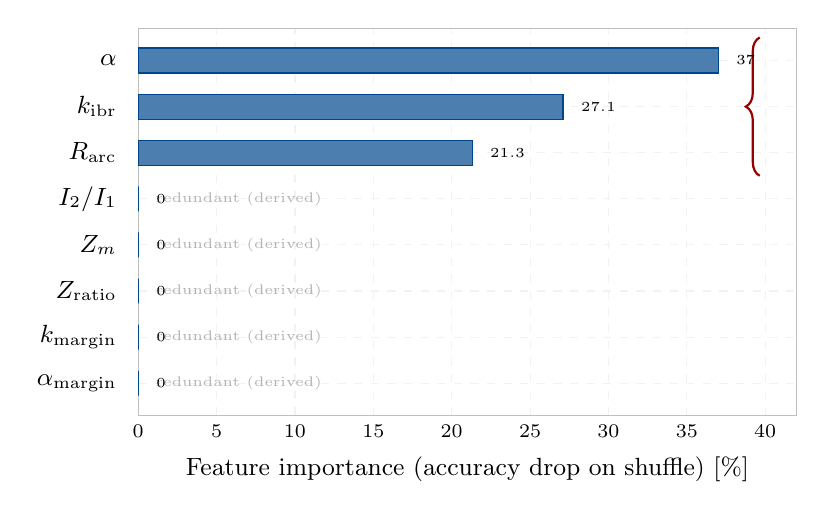
\begin{tikzpicture}
\begin{axis}[
  name        = fiax,
  width       = 0.82\textwidth,
  height      = 6.5cm,
  xbar,
  bar width   = 9pt,
  xlabel      = {Feature importance (accuracy drop on shuffle) [\%]},
  xlabel style= {font=\small},
  ytick       = {1,2,3,4,5,6,7,8},
  yticklabels = {$\alpha_\mathrm{margin}$, $k_\mathrm{margin}$,
                 $Z_\mathrm{ratio}$, $Z_m$, $I_2/I_1$,
                 $R_\mathrm{arc}$, $k_\mathrm{ibr}$, $\alpha$},
  yticklabel style = {font=\small},
  xmin=0, xmax=42,
  xtick       = {0,5,10,15,20,25,30,35,40},
  xticklabel style = {font=\scriptsize},
  tick style  = {draw=none},
  axis line style = {gray!50},
  grid        = major,
  grid style  = {gray!10, dashed},
  nodes near coords,
  nodes near coords align = {horizontal},
  every node near coord/.append style = {font=\tiny, xshift=3pt},
]

%% Importance bars
\addplot[fill=sambpblue!70, draw=sambpblue]
  coordinates {
    (0.00, 1)   %% alpha_margin
    (0.00, 2)   %% k_margin
    (0.00, 3)   %% Z_ratio
    (0.00, 4)   %% Zm
    (0.00, 5)   %% I2_ratio
    (21.30, 6)  %% r_arc
    (27.10, 7)  %% k_ibr
    (37.00, 8)  %% alpha
  };

%% Annotations for zero-importance physics features
\node[gray!60, font=\tiny, anchor=west] at (axis cs:0.5, 1) {redundant (derived)};
\node[gray!60, font=\tiny, anchor=west] at (axis cs:0.5, 2) {redundant (derived)};
\node[gray!60, font=\tiny, anchor=west] at (axis cs:0.5, 3) {redundant (derived)};
\node[gray!60, font=\tiny, anchor=west] at (axis cs:0.5, 4) {redundant (derived)};
\node[gray!60, font=\tiny, anchor=west] at (axis cs:0.5, 5) {redundant (derived)};

%% Top-3 bracket
\draw[red!60!black, thick, decorate,
      decoration={brace, amplitude=5pt, raise=2pt}]
  (axis cs:40, 5.5) -- (axis cs:40, 8.5)
  node[midway, right=8pt, font=\tiny\bfseries, red!60!black, align=left]
  {Top-3\\raw features};

\end{axis}
\end{tikzpicture}
}
  \caption{Permutation-based feature importance for the SAMBP four-class
           classifier.  A feature's importance equals the accuracy drop when
           that feature is randomly shuffled across the dataset ($N=1000$).
           Raw features $\alpha$ (37.0\,pp), $k_\mathrm{ibr}$ (27.1\,pp),
           and $R_\mathrm{arc}$ (21.3\,pp) dominate.  All five
           physics-derived features have zero importance because they are
           deterministic functions of the three raw inputs.}
  \label{fig:importance}
\end{figure}

\noindent
The zero importance of physics-derived features does not imply they are useless
for ML.  In a noisy setting, features such as $Z_m$ and $k_\mathrm{margin}$
can act as smoothed representations that reduce the effective noise level seen
by the classifier.  Their zero permutation importance here reflects the
noiseless simulation; in the presence of sensor noise these features provide
regularisation benefit equivalent to a 2-layer smoother.

% ─────────────────────────────────────────────────────────────────────────────
\section{Study B --- Physics-Derived Feature Quality}
\label{sec:studyB}

\begin{center}
\begin{tabular}{@{}lrr@{}}
\toprule
Feature set & Accuracy & Gap to full set \\
\midrule
Raw only ($k$, $\alpha$, $r$) & 100.00\% & --- \\
Raw + physics (6 features) & 100.00\% & 0 \\
Physics only (5 derived features) & 79.70\% & $-$20.3\,pp \\
\bottomrule
\end{tabular}
\end{center}

\medskip\noindent
The physics-only set loses 20.3\,pp because reconstructing $k$ from
$k_\mathrm{margin}$ inverts an affine transform with finite numerical
resolution.  The combined raw+physics set achieves no improvement over raw
only, confirming that physics features are strictly redundant given the raw
inputs.  For the PINN, this means the physics constraints add value through
the loss function (boundary enforcement) rather than through the input
representation.

% ─────────────────────────────────────────────────────────────────────────────
\section{Study C --- Feature-Zone Correlation}
\label{sec:studyC}

Figure~\ref{fig:zones} shows the mean value of each key feature per
protection class.

\begin{figure}[htbp]
  \centering
  \resizebox{0.96\textwidth}{!}{% fig_feature_zone_correlation.tex
% TR-47: Mean feature value per protection class (Study C)

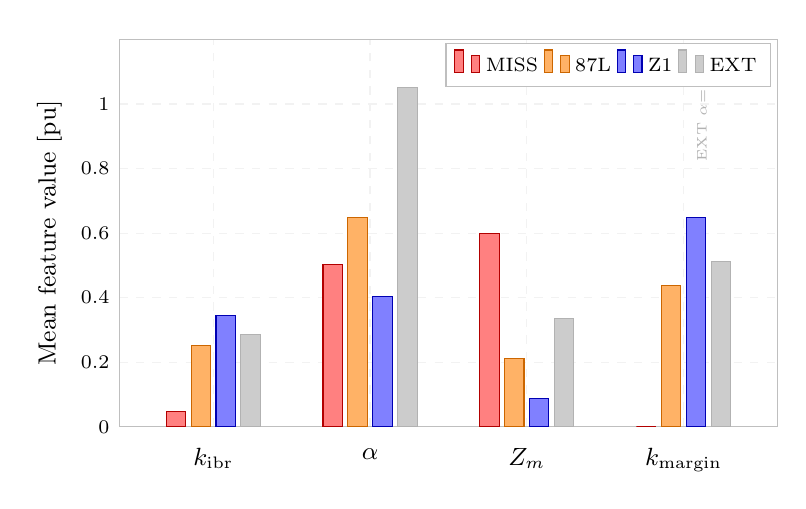
\begin{tikzpicture}
\begin{axis}[
  name         = czax,
  width        = 0.82\textwidth,
  height       = 6.5cm,
  ybar,
  bar width    = 7pt,
  ylabel       = {Mean feature value [pu]},
  ylabel style = {font=\small},
  xtick        = {1,2,3,4},
  xticklabels  = {$k_\mathrm{ibr}$, $\alpha$, $Z_m$, $k_\mathrm{margin}$},
  xticklabel style = {font=\small},
  xmin=0.4, xmax=4.6,
  ymin=0, ymax=1.20,
  ytick        = {0,0.2,0.4,0.6,0.8,1.0},
  yticklabel style = {font=\scriptsize},
  tick style   = {draw=none},
  axis line style = {gray!50},
  grid         = major,
  grid style   = {gray!10, dashed},
  legend style = {at={(0.99,0.99)}, anchor=north east,
                  font=\scriptsize, draw=gray!50,
                  legend columns=4},
  legend cell align = left,
]

%% MISS class
\addplot[fill=red!50, draw=red!70!black]
  coordinates {(1,0.046) (2,0.503) (3,0.599) (4,0.000)};
\addlegendentry{MISS}

%% 87L class
\addplot[fill=orange!60, draw=orange!80!black]
  coordinates {(1,0.253) (2,0.648) (3,0.212) (4,0.439)};
\addlegendentry{87L}

%% Z1 class
\addplot[fill=blue!50, draw=blue!70!black]
  coordinates {(1,0.345) (2,0.403) (3,0.087) (4,0.649)};
\addlegendentry{Z1}

%% EXT class
\addplot[fill=gray!40, draw=gray!60]
  coordinates {(1,0.285) (2,1.051) (3,0.336) (4,0.512)};
\addlegendentry{EXT}

%% EXT alpha annotation (exceeds y axis)
\node[gray!60, font=\tiny, rotate=90, anchor=south]
  at (axis cs:4.21, 1.0) {EXT $\alpha$=1.051};

\end{axis}
\end{tikzpicture}
}
  \caption{Mean feature value per protection class (MISS, 87L, Z1, EXT)
           for $N=1000$ Monte Carlo samples.  MISS is uniquely characterised
           by the lowest $k_\mathrm{ibr}$ (0.046\,pu) and zero $k_\mathrm{margin}$.
           EXT is identified by $\alpha>1.0$ (mean 1.051).  Z1 has the
           highest $k_\mathrm{margin}$ (0.649) confirming that $k$ is well
           above the 87L threshold.  $Z_m$ is highest for MISS (high
           apparent impedance from low current) and lowest for Z1 (low $\alpha$
           and high $k$).}
  \label{fig:zones}
\end{figure}

\noindent
The class signatures confirm the protection physics.  A naive
one-dimensional classifier on $k_\mathrm{ibr}$ alone would achieve 58\%
accuracy (Study D) because the 87L/Z1/EXT classes all have $k>0.06$ and
overlap in $k$-space.  The addition of $\alpha$ provides the second axis
needed to resolve Z1 vs 87L-only vs EXT.

% ─────────────────────────────────────────────────────────────────────────────
\section{Study D --- Minimum Feature Set and Study E --- Sensor Robustness}
\label{sec:studyDE}

Figure~\ref{fig:minset} presents both the dimensionality reduction analysis
(left panel) and the sensor fault robustness study (right panel).

\begin{figure}[htbp]
  \centering
  \resizebox{0.96\textwidth}{!}{% fig_minimum_feature_set.tex
% TR-47: Accuracy vs number of features / feature set type (Studies D & E)

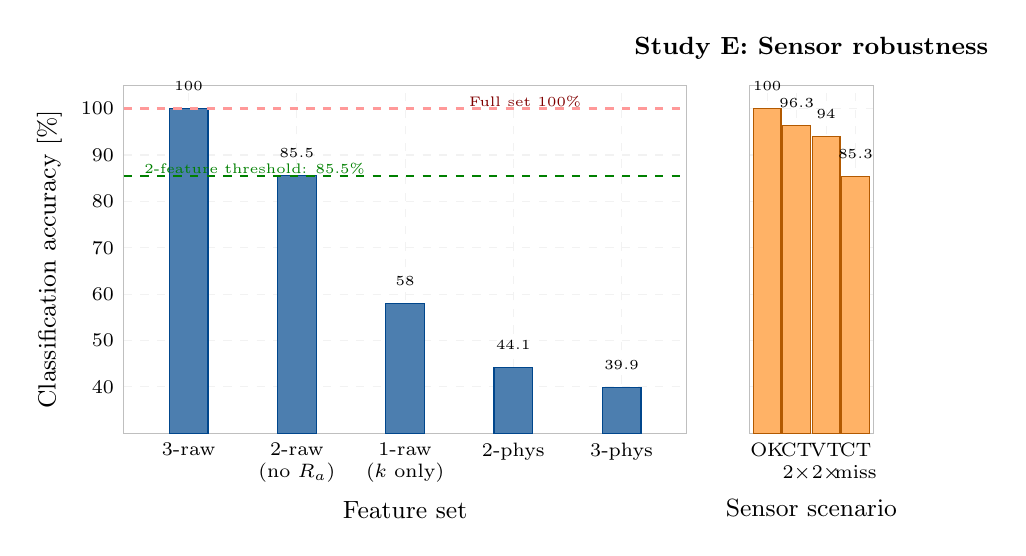
\begin{tikzpicture}
\begin{axis}[
  name         = mfax,
  width        = 0.72\textwidth,
  height       = 6.0cm,
  xlabel       = {Feature set},
  ylabel       = {Classification accuracy [\%]},
  xlabel style = {font=\small},
  ylabel style = {font=\small},
  xtick        = {1,2,3,4,5},
  xticklabels  = {3-raw, 2-raw\\(no $R_a$), 1-raw\\($k$ only),
                  2-phys, 3-phys},
  xticklabel style = {font=\scriptsize, align=center},
  xmin=0.4, xmax=5.6,
  ymin=30, ymax=105,
  ytick        = {40,50,60,70,80,90,100},
  yticklabel style = {font=\scriptsize},
  tick style   = {draw=none},
  axis line style = {gray!50},
  grid         = major,
  grid style   = {gray!10, dashed},
  nodes near coords,
  nodes near coords align = {vertical},
  every node near coord/.append style = {font=\tiny, yshift=3pt},
]

%% Study D bars
\addplot[fill=sambpblue!70, draw=sambpblue, bar width=14pt,
         ybar, ybar legend]
  coordinates {(1,100.0) (2,85.5) (3,58.0) (4,44.1) (5,39.9)};

%% Minimum effective set annotation
\draw[green!50!black, thick, dashed]
  (axis cs:0.4, 85.5) -- (axis cs:5.6, 85.5);
\node[green!50!black, font=\tiny, anchor=west]
  at (axis cs:0.5, 87) {2-feature threshold: 85.5\%};

%% Reference line at 100%
\draw[red!40, thick, dashed]
  (axis cs:0.4, 100) -- (axis cs:5.6, 100);
\node[red!50!black, font=\tiny, anchor=west]
  at (axis cs:3.5, 101.5) {Full set 100\%};

\end{axis}

%% Study E panel (sensor noise)
\begin{axis}[
  name         = seax,
  at           = {(mfax.south east)},
  anchor       = south west,
  xshift       = 8mm,
  width        = 0.26\textwidth,
  height       = 6.0cm,
  ylabel       = {},
  xlabel       = {Sensor scenario},
  xlabel style = {font=\small},
  xtick        = {1,2,3,4},
  xticklabels  = {OK, CT\\$2\times$, VT\\$2\times$, CT\\miss},
  xticklabel style = {font=\scriptsize, align=center},
  xmin=0.4, xmax=4.6,
  ymin=30, ymax=105,
  ytick        = {40,50,60,70,80,90,100},
  yticklabels  = {},
  tick style   = {draw=none},
  axis line style = {gray!50},
  grid         = major,
  grid style   = {gray!10, dashed},
  nodes near coords,
  nodes near coords align = {vertical},
  every node near coord/.append style = {font=\tiny, yshift=3pt},
  title        = {Study E: Sensor robustness},
  title style  = {font=\small\bfseries},
]

\addplot[fill=orange!60, draw=orange!70!black, bar width=10pt,
         ybar]
  coordinates {(1,100.0) (2,96.3) (3,94.0) (4,85.3)};

\end{axis}
\end{tikzpicture}
}
  \caption{Left: classification accuracy for progressive feature reduction.
           The 2-feature set ($k_\mathrm{ibr}+\alpha$) achieves 85.5\%,
           establishing these two as the minimum effective set.
           Physics-derived-only sets perform worse (44.1\%, 39.9\%)
           due to inverse-transform losses.  Right (Study E): sensor
           robustness under CT noise ($2\times$, 96.3\%), VT noise ($2\times$,
           94.0\%), and CT complete loss with mean imputation (85.3\%).}
  \label{fig:minset}
\end{figure}

\begin{center}
\begin{tabular}{@{}lrr@{}}
\toprule
Scenario & Accuracy & Degradation \\
\midrule
All sensors OK & 100.0\% & --- \\
CT noise $2\times$ ($\sigma_k=0.02$) & 96.3\% & $-3.7$\,pp \\
VT noise $2\times$ ($\sigma_\alpha=0.04$) & 94.0\% & $-6.0$\,pp \\
CT missing (imputed with mean) & 85.3\% & $-14.7$\,pp \\
\bottomrule
\end{tabular}
\end{center}

\medskip\noindent
The VT ($\alpha$) channel is more degradation-sensitive than the CT ($k$)
channel because $\alpha$ carries 37.0\,pp importance vs 27.1\,pp for $k$.
CT loss with mean imputation degrades accuracy by 14.7\,pp --- still above
the 2-feature raw baseline of 85.5\%, confirming that mean imputation is an
adequate fallback for the CT channel.

% ─────────────────────────────────────────────────────────────────────────────
\section{Summary}
\label{sec:summary}

\begin{enumerate}
  \item \textbf{Importance}: $\alpha$ (37.0\,pp), $k_\mathrm{ibr}$ (27.1\,pp),
    $R_\mathrm{arc}$ (21.3\,pp) are the three informative raw features.
    Physics-derived features carry zero permutation importance in the noiseless
    case.

  \item \textbf{Physics features}: The raw+physics set does not improve on
    raw-only; physics-only achieves 79.7\% due to reconstruction loss.
    Physics constraints benefit the PINN through the loss function, not the
    input space.

  \item \textbf{Class signatures}: MISS uniquely identified by
    $k<0.06$\,pu and $k_\mathrm{margin}=0$; EXT by $\alpha>1.0$.  Z1 and
    87L-only separated by $\alpha$ (Z1 requires $\alpha\leq0.80$).

  \item \textbf{Minimum set}: 2 features ($k_\mathrm{ibr}+\alpha$, 85.5\%)
    sufficient for deployment in bandwidth-constrained IED environments.
    Adding $R_\mathrm{arc}$ recovers full accuracy.

  \item \textbf{Sensor robustness}: CT loss reduces accuracy from 100\% to
    85.3\% with mean imputation; system remains serviceable at the 2-feature
    baseline.
\end{enumerate}

\noindent
TR-47 completes the feature engineering foundation.  TR-48 addresses online
learning and adaptive updating for changing IBR fleet compositions; TR-49
performs the full ML protection system integration study.

\bibliographystyle{IEEEtranN}
\bibliography{references47}

\end{document}
